\documentclass[tikz]{standalone}
\usepackage{pgfplots}
\usepackage{mathptmx}
\usepackage{ctex}
% \pgfplotsset{compat=1.16}
\begin{document}
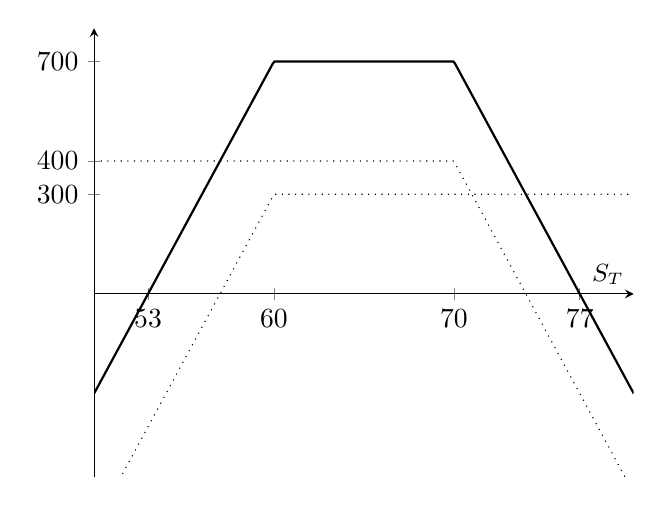
\begin{tikzpicture}
    \begin{axis}[
        axis lines = middle,
        xlabel = {$S_T$},
        ymin=-550, ymax=800,
        xmin=50, xmax=80,
        scaled x ticks=false,
        xtick={77, \KP, \KC, 53},
        ytick={700, 400, 300},
        % width=10cm,
        % height=7cm,
        % axis equal,
        label style={font=\small}
    ]
    % 定义参数
    \def\St{65}  % 期权费
    \def\KC{70}
    \def\KP{60}
    \def\PC{4}
    \def\PP{3}
    \def\MUL{100}
    
    % 绘制看涨期权到期收益曲线
    \addplot[domain=50:80,dotted,samples=300] {(min(0, \KC-x)+\PC)*\MUL};
    \addplot[domain=50:80,dotted,samples=300] {(min(0, x-\KP)+\PP)*\MUL};
    \addplot[domain=50:80,samples=300, thick] {(min(0, \KC-x)+\PC+min(0, x-\KP)+\PP)*\MUL};
    \end{axis}
\end{tikzpicture}

\end{document}